\documentclass{article}
\pdfpagewidth=8.5in
\pdfpageheight=11in

\usepackage{ijcai26}
\usepackage{times}
\usepackage{soul}
\usepackage{url}
\usepackage[hidelinks]{hyperref}
\usepackage[utf8]{inputenc}
\usepackage[small]{caption}
\usepackage{graphicx}
\usepackage{amsmath}
\usepackage{amssymb}
\usepackage{booktabs}
\usepackage{multirow}
\usepackage[switch]{lineno}

\linenumbers
\urlstyle{same}

\pdfinfo{
/TemplateVersion (IJCAI.2026.0)
}

\title{Counterfactual Structural Sensitivity: Dataset-Only Diagnostics for Negation and Argument-Role Consistency in Language Model Representations}

\author{Anonymous Submission}

\begin{document}

\maketitle

\begin{abstract}
We introduce Counterfactual Structural Sensitivity (CSS), a dataset-only protocol for testing whether language-model hidden states respond systematically to minimal structural edits. CSS compares each sentence with a counterfactual variant and measures layer-wise representation shifts for role reversal and negation. Unlike output-only minimal-pair tests, CSS evaluates internal geometry using centroid cosine, Frobenius-style token-matrix similarity, L2 distance, and token-aligned shift, then relates these shifts to GPT-2 autoregressive surprisal, linear-probe selectivity, qualitative audits, and forced-choice output consistency. On 3,000 psycholinguistic counterfactual pairs, BERT, RoBERTa, and GPT-2 show broad positive shift-surprisal association for cosine and Frobenius metrics, and Frobenius adds positive adjusted-$R^2$ beyond cosine in 70/78 baseline layer/model/phenomenon cells. Modern decoder extensions with Mistral-7B-Instruct and Gemma-3-4B-IT show that identity judgments are near perfect, but counterfactual rejection remains imperfect, especially for negation. The results support CSS as a reproducible diagnostic for structural and logical sensitivity, not as evidence that model processing is human-like.
\end{abstract}

\section{Introduction}

Large language models often behave as if they understand syntactic and semantic structure, yet small structural edits can alter meaning in ways that surface-level overlap does not reveal. For example, \emph{the chef praised the waiter} and \emph{the waiter praised the chef} contain the same main lexical items but reverse the event participants. Similarly, adding \emph{not} changes a polarity relation even when the surrounding sentence remains mostly unchanged. These edits are central to logical and symbolic reasoning because they probe argument-role consistency, polarity sensitivity, and the stability of representations under controlled counterfactuals.

Existing minimal-pair evaluations have shown that language models can be sensitive to some grammatical contrasts while remaining brittle on others \cite{warstadt2020blimp,ettinger2020bert,shivagunde2023larger}. However, output accuracy alone does not reveal whether a model's internal states undergo a systematic structural change. Conversely, probing hidden states without a controlled counterfactual may conflate linguistic structure with lexical frequency, sentence length, or template artifacts.

We propose Counterfactual Structural Sensitivity (CSS), a protocol that asks: \emph{when a sentence undergoes a minimal structural edit, do layer-wise representations move in a systematic way, and are different geometric metrics complementary?} The current study is deliberately dataset-only: it does not depend on new human annotations and does not claim human-like comprehension. Instead, it tests whether hidden-state shifts are consistent across edit types, layers, model families, and metrics, and whether these shifts relate to autoregressive surprisal and output-level consistency.

Our contributions are:
\begin{itemize}
    \item A reproducible CSS pipeline for role reversal and negation: sentence pair construction, hidden-state extraction, layer-wise metrics, probes, surprisal, and dataset-level statistics.
    \item A matrix-norm adaptation for contextual token matrices, motivated by matrix-norm document similarity \cite{vonderbruck2019matrix}, and compared directly against centroid cosine.
    \item A full baseline study over BERT, RoBERTa, and GPT-2, plus modern decoder extensions with Mistral-7B-Instruct and Gemma-3-4B-IT.
    \item A forced-choice output-consistency diagnostic showing that modern instruction models handle identity controls but still fail on a nontrivial fraction of counterfactual role and negation pairs.
    \item A qualitative audit linking aggregate patterns to concrete sentence pairs and dataset artifacts, which keeps the claims conservative and interpretable.
\end{itemize}

\section{Related Work}

\paragraph{Minimal pairs and psycholinguistic diagnostics.}
BLiMP established large-scale minimal-pair evaluation for grammatical knowledge \cite{warstadt2020blimp}. Ettinger's psycholinguistic diagnostics showed that BERT captures some role and event cues but remains weak on negation and other semantic phenomena \cite{ettinger2020bert}. Shivagunde et al. extend such diagnostics to larger role-reversal and negation datasets, which we use as the source of controlled counterfactual pairs \cite{shivagunde2023larger}. CSS builds on this line by shifting the target from output-only accuracy to layer-wise hidden-state response under paired counterfactual edits.

\paragraph{Representation probing.}
Probing studies test whether linguistic properties are recoverable from hidden states \cite{conneau2018senteval,tenney2019bert}. Hewitt and Liang caution that probe accuracy alone can reflect probe capacity or dataset artifacts, motivating random-label controls and selectivity measures \cite{hewitt2019designing}. We therefore use linear probes as secondary diagnostics and report selectivity rather than treating probe accuracy as direct evidence of encoded structure.

\paragraph{Similarity, matrix norms, and surprisal.}
Centroid cosine similarity is common for sentence-level embedding comparison, but it can discard token-token relational structure. vor der Bruck and Pouly show that matrix norms can improve document similarity with static word embeddings \cite{vonderbruck2019matrix}. We adapt this idea to contextual token matrices. Separately, surprisal provides a probabilistic predictor of processing difficulty in psycholinguistics \cite{levy2008expectation}. We use GPT-2 left-to-right surprisal \cite{radford2019language}; masked-LM pseudo-log-likelihood \cite{salazar2020masked} is conceptually different and is not used as the primary surprisal measure.

\section{CSS Protocol}

Let $s$ be a sentence and $s'=T_{\mathrm{edit}}(s)$ be a counterfactual sentence produced by a controlled structural edit. CSS extracts hidden states from a model $f_\theta$ for every layer $l$:
\begin{equation}
    H_l(s) \in \mathbb{R}^{n \times d}, \qquad H_l(s') \in \mathbb{R}^{m \times d},
\end{equation}
where rows are word-level vectors after mean pooling subword pieces. Sentence vectors are obtained by mean pooling word vectors:
\begin{equation}
    \bar{h}_l(s) = \frac{1}{n}\sum_{i=1}^{n}H_l(s)_i .
\end{equation}
The pipeline is:
\[
\text{sentence} \rightarrow \text{counterfactual edit} \rightarrow \text{hidden states} \rightarrow \text{shift metrics} \rightarrow \text{probes + surprisal} \rightarrow \text{analysis}.
\]

\subsection{Phenomena}

We use two primary edit types. \textbf{Role reversal} swaps event participants or argument roles while preserving much of the lexical material. These examples test argument-role and event-structure consistency. \textbf{Negation} compares affirmative and negated variants, testing polarity sensitivity and negation consistency. Attachment ambiguity is not included in the primary study because the current dataset-only claim requires clean source coverage and surface controls.

\subsection{Representation-Shift Metrics}

CSS computes four layer-wise shifts for every pair, model, and phenomenon.

\paragraph{Centroid cosine shift.}
\begin{equation}
    \Delta^{\mathrm{cos}}_l(s,s') =
    1 - \cos(\bar{h}_l(s), \bar{h}_l(s')) .
\end{equation}
This is the simplest sentence-level movement measure. It is robust and interpretable, but it compresses the entire sentence into one vector.

\paragraph{Frobenius token-matrix shift.}
Let $A_l$ and $B_l$ be row-normalized word-level matrices for $s$ and $s'$. We define:
\begin{equation}
    \mathrm{sim}^{\mathrm{frob}}_l =
    \frac{\|K(A_lB_l^\top)\|_F}
    {\sqrt{\|K(A_lA_l^\top)\|_F\|K(B_lB_l^\top)\|_F + \epsilon}},
\end{equation}
\begin{equation}
    \Delta^{\mathrm{frob}}_l = 1 - \mathrm{sim}^{\mathrm{frob}}_l .
\end{equation}
Here $K(\cdot)$ denotes the pairwise similarity matrix after masking or alignment choices. Unlike centroid cosine, this metric can respond to changes in the relational geometry among contextual token vectors.

\paragraph{L2 shift.}
\begin{equation}
    \Delta^{\mathrm{L2}}_l(s,s') =
    \|\bar{h}_l(s)-\bar{h}_l(s')\|_2 .
\end{equation}
L2 preserves raw magnitude information, but its scale is model-dependent.

\paragraph{Token-aligned shift.}
For an alignment $\mathcal{A}$ between tokens in the two sentences:
\begin{equation}
    \Delta^{\mathrm{tok}}_l =
    \frac{1}{|\mathcal{A}|}\sum_{(i,j)\in\mathcal{A}}
    \left(1-\cos(H_l(s)_i,H_l(s')_j)\right).
\end{equation}
This metric is local and token-sensitive, but it can become unstable when the edit changes length or introduces difficult alignments.

\section{Experimental Setup}

\subsection{Data}

We use the public role-reversal and negation datasets of Shivagunde et al. \cite{shivagunde2023larger}. The final CSS dataset contains 1,500 role-reversal pairs and 1,500 negation pairs. For each pair we store the original sentence, counterfactual sentence, phenomenon, edit type, edited spans, split, lexical Jaccard, length differences, edit distance, source metadata, and schema version. The role data are drawn from ROLE-1500. The negation data are drawn from NEG-1500-SIMP-GEN. We include both directions where the source pair supports them, so negation includes insertion and removal views.

The dataset is intentionally controlled but not artifact-free. Our qualitative audit finds that role reversal has higher lexical overlap and nearly zero length change, while negation often combines a negation cue with a predicate or category foil. This matters for interpretation: mean shift magnitude and rank correlation need not agree.

\subsection{Models}

The primary baseline models are BERT-base-uncased \cite{devlin2019bert}, RoBERTa-base \cite{liu2019roberta}, and GPT-2 \cite{radford2019language}. For each baseline we extract the embedding layer plus 12 transformer layers. We also run regular-paper extensions on Mistral-7B-Instruct-v0.3 \cite{jiang2023mistral} and Gemma-3-4B-IT \cite{gemmateam2025gemma3}, extracting all available hidden layers. All models are run in evaluation mode with hidden-state output enabled.

\subsection{Surprisal}

For each sentence, GPT-2 token surprisal is:
\begin{equation}
    \mathrm{surprisal}(w_i) = -\log p(w_i \mid w_1,\ldots,w_{i-1}).
\end{equation}
We report total surprisal, average surprisal, counterfactual minus original surprisal, absolute surprisal difference, and edited-region surprisal when span coverage permits. Surprisal is treated as a probabilistic covariate, not as a complete model of comprehension.

\subsection{Probes}

Linear probes are trained by layer for role and negation properties. Each probe is paired with random-label controls, and selectivity is measured as the difference between task macro-F1 and control macro-F1. This follows the control-task warning of Hewitt and Liang \cite{hewitt2019designing}. We use probes as a secondary diagnostic because high recoverability does not by itself establish that the model uses the encoded property.

\subsection{Output-Level Consistency}

For GPT-2, Mistral, and Gemma, we also run a forced-choice yes/no diagnostic. Identity controls ask whether a sentence is consistent with itself, where the expected answer is yes. Counterfactual prompts ask whether the edited sentence preserves the same event or proposition, where the expected answer is no. This is a behavioral diagnostic of counterfactual sensitivity, not a full test of logical reasoning.

\subsection{Statistics}

The primary dataset-only statistic is Spearman correlation between a layer-wise shift metric and absolute GPT-2 average-surprisal delta. Pearson correlation is secondary. We compute bootstrap confidence intervals and Benjamini-Hochberg FDR correction across layer-wise tests. Frobenius complementarity is tested by comparing adjusted-$R^2$ for a regression target using cosine alone versus cosine plus Frobenius:
\begin{equation}
    \Delta R^2_{\mathrm{adj}} =
    R^2_{\mathrm{adj}}(y \sim \Delta^{\mathrm{cos}}+\Delta^{\mathrm{frob}})
    - R^2_{\mathrm{adj}}(y \sim \Delta^{\mathrm{cos}}).
\end{equation}

\begin{table}[t]
\centering
\small
\begin{tabular}{lrrrr}
\toprule
Artifact & Role & Neg. & Models & Rows \\
\midrule
Input pairs & 1500 & 1500 & -- & 3000 \\
Baseline hidden metrics & 1500 & 1500 & 3 & 117000 \\
Mistral hidden metrics & 1500 & 1500 & 1 & 99000 \\
Gemma hidden metrics & 1500 & 1500 & 1 & 105000 \\
GPT-2 surprisal & 1500 & 1500 & 1 & 3000 \\
Probe summaries & -- & -- & 3 & 390 \\
\bottomrule
\end{tabular}
\caption{Coverage of the current CSS study. Baseline rows equal 3,000 pairs $\times$ 3 models $\times$ 13 layers. Modern decoder rows use all available hidden layers.}
\label{tab:coverage}
\end{table}

\section{Results}

\subsection{RQ1: Are representation shifts systematic?}

Across the three baseline models, cosine, Frobenius, and L2 shifts show broad positive association with GPT-2 surprisal deltas. Table~\ref{tab:rq1} summarizes significant cells after FDR correction. Frobenius has the highest number of positive significant cells (52/78), followed by cosine (50/78) and L2 (47/78). Token-aligned shift is more mixed, with equal numbers of positive and negative significant cells.

\begin{table}[t]
\centering
\small
\begin{tabular}{lrrrr}
\toprule
Metric & Cells & Pos. sig. & Neg. sig. & Pos. rate \\
\midrule
$\Delta^{\mathrm{cos}}$ & 78 & 50 & 6 & 0.641 \\
$\Delta^{\mathrm{frob}}$ & 78 & 52 & 6 & 0.667 \\
$\Delta^{\mathrm{L2}}$ & 78 & 47 & 5 & 0.603 \\
$\Delta^{\mathrm{tok}}$ & 78 & 32 & 32 & 0.410 \\
\bottomrule
\end{tabular}
\caption{Baseline significant shift-surprisal cells after FDR correction across 3 models, 2 phenomena, and 13 layers.}
\label{tab:rq1}
\end{table}

The layer profiles differ by phenomenon. For Frobenius shift, negation peaks at the embedding layer for all three baseline models: BERT $\rho=0.154$, GPT-2 $\rho=0.131$, and RoBERTa $\rho=0.118$. Role reversal peaks in middle-to-late layers: BERT layer 7 with $\rho=0.329$, RoBERTa layer 7 with $\rho=0.368$, and GPT-2 layer 10 with $\rho=0.318$. This supports the claim that different structural edits produce phenomenon-specific layer signatures.

\begin{figure}[t]
\centering
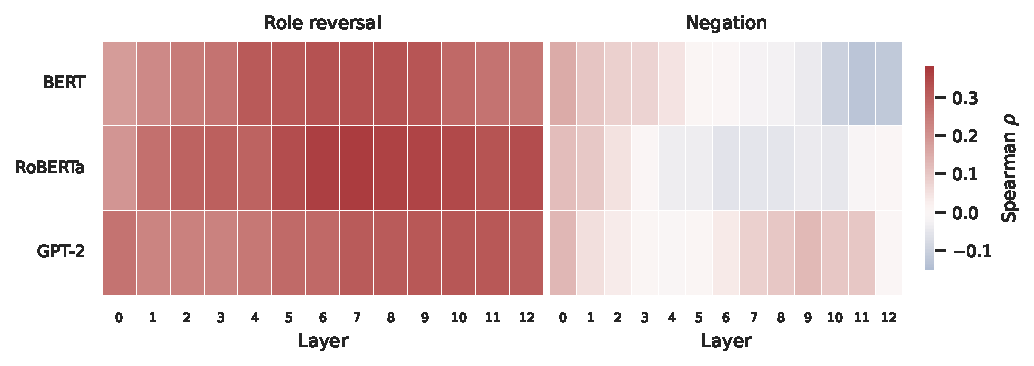
\includegraphics[width=\columnwidth]{figures/baseline_frob_layer_heatmap.pdf}
\caption{Baseline layer-wise Spearman correlations for Frobenius shift. Role reversal shows stronger mid-to-late layer alignment, while negation peaks earlier.}
\label{fig:baseline_heatmap}
\end{figure}

\subsection{RQ2: Does Frobenius add value beyond cosine?}

Frobenius shift adds complementary information beyond centroid cosine. In the baseline study, adding Frobenius to cosine gives positive adjusted-$R^2$ gain in 70/78 layer/model/phenomenon cells, with mean $\Delta R^2_{\mathrm{adj}}=0.0114$. The gain is modest but consistent, which is the important point: Frobenius should not be framed as universally superior, but as a metric that captures token-matrix geometry not available to a single pooled vector.

\begin{figure}[t]
\centering
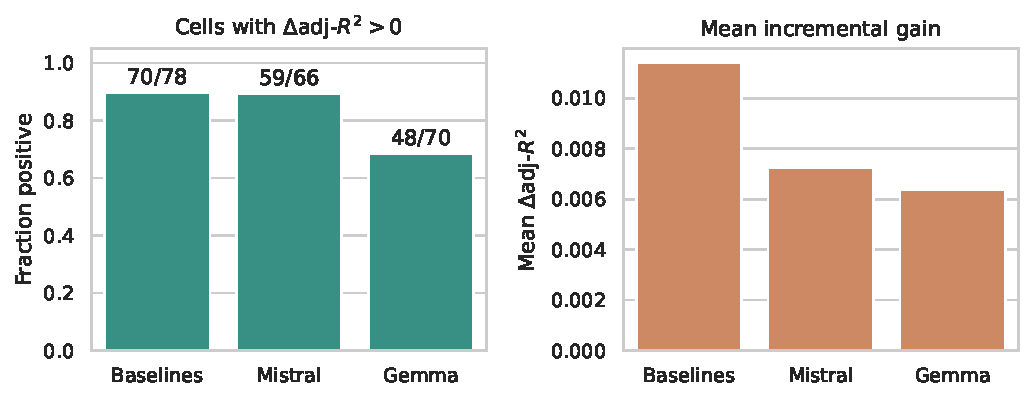
\includegraphics[width=\columnwidth]{figures/frob_incremental_comparison.pdf}
\caption{Frobenius complementarity. The left panel shows the fraction of cells with positive adjusted-$R^2$ gain after adding Frobenius beyond cosine. The right panel shows mean gain.}
\label{fig:frob_incremental}
\end{figure}

\subsection{RQ3: Do probes and surprisal provide redundant signals?}

Probe selectivity is consistently positive, with mean selectivity approximately 0.51 macro-F1 over random-label controls. However, the layer-wise coupling between probe selectivity and shift-surprisal correlation is weak: for Frobenius, Spearman correlation is approximately $-0.011$ and Pearson correlation is approximately $0.013$. This suggests that probes and CSS shifts are complementary. A probe can recover a label from hidden states without showing that pair-level representation movement tracks probabilistic difficulty, and a shift metric can track pair-level movement without requiring high probe selectivity.

\subsection{RQ4: Do modern decoder outputs preserve counterfactual consistency?}

Figure~\ref{fig:output_consistency} shows that instruction-tuned decoders solve identity controls but still fail on meaningful counterfactuals. Mistral reaches 1.000 identity accuracy for both phenomena, but only 0.734 role-reversal rejection and 0.652 negation rejection. Gemma reaches 0.999 role identity and 1.000 negation identity, with stronger but still imperfect counterfactual rejection: 0.969 for role reversal and 0.814 for negation. GPT-2 is not a reliable behavioral comparator because its identity controls are poor; it is retained for left-to-right surprisal and as a biased output baseline.

\begin{figure}[t]
\centering
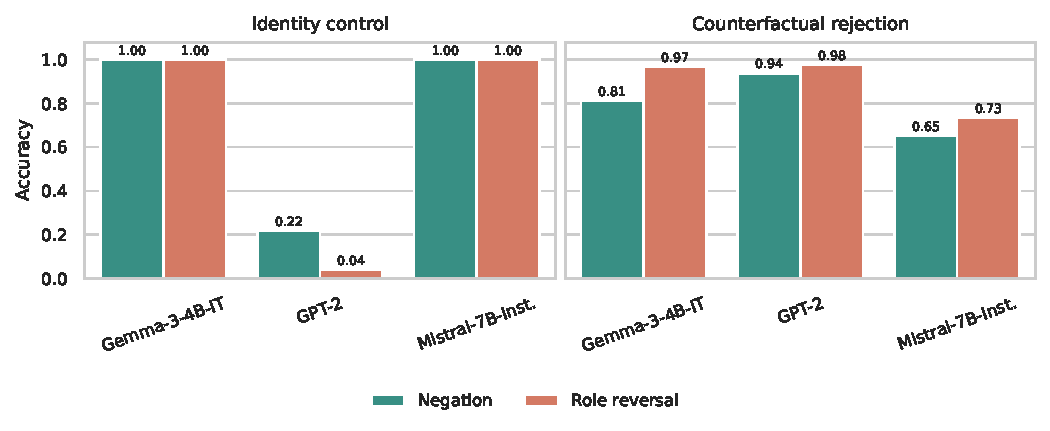
\includegraphics[width=\columnwidth]{figures/output_consistency_accuracy.pdf}
\caption{Forced-choice output consistency. Identity controls verify prompt usability for instruction models. Counterfactual rejection reveals remaining sensitivity gaps, especially for negation.}
\label{fig:output_consistency}
\end{figure}

\subsection{RQ5: Do modern decoders show CSS-style hidden sensitivity?}

The modern decoder hidden-state extension confirms that CSS patterns are not limited to the three small baselines. Mistral produces 99,000 metric rows with no Frobenius warnings; Gemma produces 105,000 rows with no Frobenius warnings. Mistral's strongest Frobenius-surprisal alignment is role reversal at layer 6 ($\rho=0.324$, FDR $q=1.15\times 10^{-35}$), and negation at layer 0 ($\rho=0.175$, $q=2.31\times 10^{-11}$). Gemma's strongest role-reversal alignment is also layer 6 ($\rho=0.319$, $q=2.25\times 10^{-34}$), while its strongest negation alignment appears at layer 4 ($\rho=0.145$, $q=4.27\times 10^{-8}$).

\begin{figure}[t]
\centering
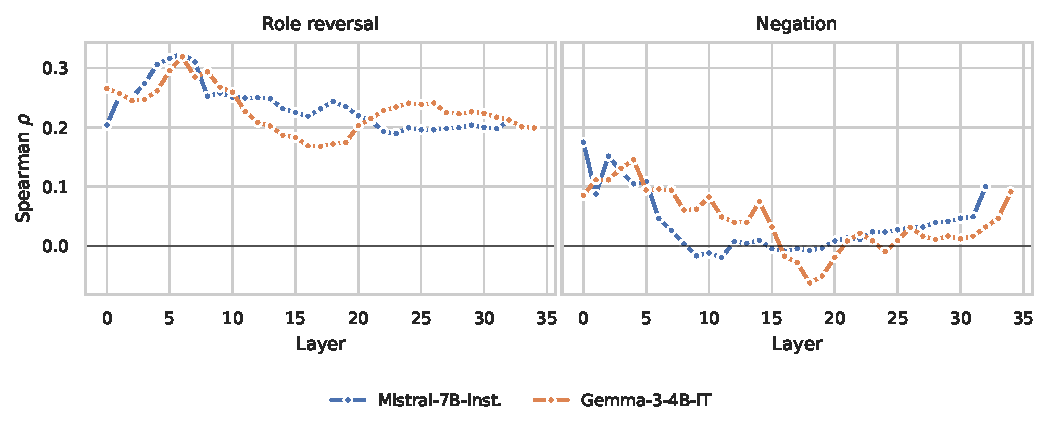
\includegraphics[width=\columnwidth]{figures/modern_decoder_frob_curves.pdf}
\caption{Modern decoder Frobenius-shift correlations with GPT-2 surprisal. Role reversal has a clear early-to-middle layer peak in both Mistral and Gemma; negation is weaker and earlier.}
\label{fig:modern_curves}
\end{figure}

Frobenius complementarity also transfers to these larger decoders: adjusted-$R^2$ gain is positive in 59/66 Mistral cells and 48/70 Gemma cells. The lower Gemma positive rate suggests model-specific geometry and scaling effects, so the correct interpretation is complementarity rather than universal dominance.

\section{Qualitative Analysis}

Aggregate curves can obscure why role reversal and negation behave differently. We therefore inspect representative cases selected by high/low Frobenius shift and high/low absolute surprisal delta. The main pattern is that mean shift magnitude and correlation answer different questions. Mean shift asks how far representations move on average; correlation asks whether item-level movement ranks align with surprisal deltas.

Negation has lower lexical overlap and larger length differences than role reversal. Its mean lexical Jaccard is 0.485, mean absolute length delta is 1.001, and mean Frobenius shift is 0.058 in the baseline aggregate. Role reversal has mean lexical Jaccard 0.797, mean absolute length delta 0.047, and mean Frobenius shift 0.020. Thus negation can have larger average displacement because many examples change both polarity and category predicate, while role reversal can show cleaner rank alignment despite smaller average magnitude.

Representative examples illustrate the dissociation. In one high-shift but low-surprisal negation case, \emph{A hammer is an instrument} becomes \emph{A hammer is not a dessert}. The hidden-state geometry moves strongly, but the average surprisal delta is near zero. In a low-shift but high-surprisal role case, \emph{The cashier counted which bills the robber had given} becomes \emph{The cashier counted which robber the bills had given}. GPT-2 surprisal changes sharply, but averaged representation movement is small. These cases show why CSS should remain a multi-diagnostic framework.

The qualitative audit also exposes source-data artifacts, including article mismatches, category-foil substitutions, and implausible role continuations. These artifacts do not invalidate the controlled diagnostic, but they narrow the claim: CSS supports dataset-level representational and behavioral sensitivity analysis, not a direct claim about human semantic judgments.

\section{Discussion}

CSS is useful because it separates three questions that are often conflated. First, does an edit move hidden representations? Second, does the movement rank-align with a probabilistic signal such as surprisal? Third, does the model behaviorally reject the counterfactual as meaning-preserving? Our results show that these are related but not identical. Role reversal tends to produce cleaner layer-wise correlation patterns, while negation often induces larger raw shifts but noisier interpretation because the source examples include lexical and category changes.

The Frobenius result is important but should be stated carefully. The mean adjusted-$R^2$ gain is not large, but it is positive across most cells and persists in modern decoder extensions. This supports the hypothesis that token-token relational geometry carries information beyond a sentence centroid. It does not prove that Frobenius is always the best metric, nor that it captures logical structure in isolation.

For the LogiSymb setting, the output-consistency experiment is the strongest behavioral bridge. Instruction models can say that identical sentences are equivalent, which verifies the prompt format, yet still fail on counterfactual edits. Gemma is substantially stronger than Mistral, but negation remains harder than role reversal. This aligns with the broader observation that logical polarity is not solved by surface fluency alone.

\section{Limitations}

The study is dataset-only and does not include new human annotations. Therefore, we do not claim human alignment or human-like processing. The dataset is generated and contains artifacts, so all item-level examples are diagnostic rather than naturalistic. The output-consistency test is a constrained yes/no prompt and should not be overinterpreted as a full logical reasoning benchmark. The main baseline models are small by 2026 standards, although we include two modern decoder extensions. Finally, CSS is correlational: it identifies systematic movement but does not causally prove which hidden dimensions or attention patterns implement structural reasoning.

\section{Conclusion}

Counterfactual Structural Sensitivity provides a reproducible way to analyze how language-model representations react to controlled structural edits. Across role reversal and negation, hidden-state shifts are systematic, layer profiles differ by phenomenon, Frobenius token-matrix geometry adds complementary value beyond centroid cosine, and modern decoder outputs still show counterfactual consistency gaps. The strongest defensible conclusion is not that language models process sentences like humans, but that controlled counterfactual edits reveal measurable and interpretable structural sensitivity in both hidden states and model behavior.

\bibliographystyle{named}
\bibliography{css_logisymb_2026_regular}

\end{document}
